\section{model}

We propose a deep neural model to capture linguistics partern of the text. This model is based on simple Convolutional Neural Network with an embedding layer for words representaion, one covolutional with pooling layer and finnaly one Dense layer. Figure \ref{cnn} shows the global structure of our architecture. The input is a sequence of words $ w_{1}, w_{2} ... w_{n} $ and the output is class (for text classification). The embedding is build on top of a Word2Vec architecture trained on a Skip-gram model. Our text tokenizer keeps all the words, event if a words are rare, to make sure all linguistics material could be detected at the end by the model. This kind of embedding give us a good starting point for the word represention in vector, but we make it trainable also by the model to reach the best text-classification acuracy. 

The Convolutional layer is based on 2 dimensional convolutions, the same as we use for pictures convolutions, but with a fixed width corresponding to the max width represented by the embedding size. At the end we transform the 2 dimensional convolutions in 1 dimensional convolution. The common convolution used in general for the text. The only parameter we can modify here is the height of the filter corresponding to the number of words we want to put in the filter. The goal of this approach is to use the standard picture deconvolution (conv2D Transpose) for our model fit on text.

\begin{figure}[h]
\begin{center}
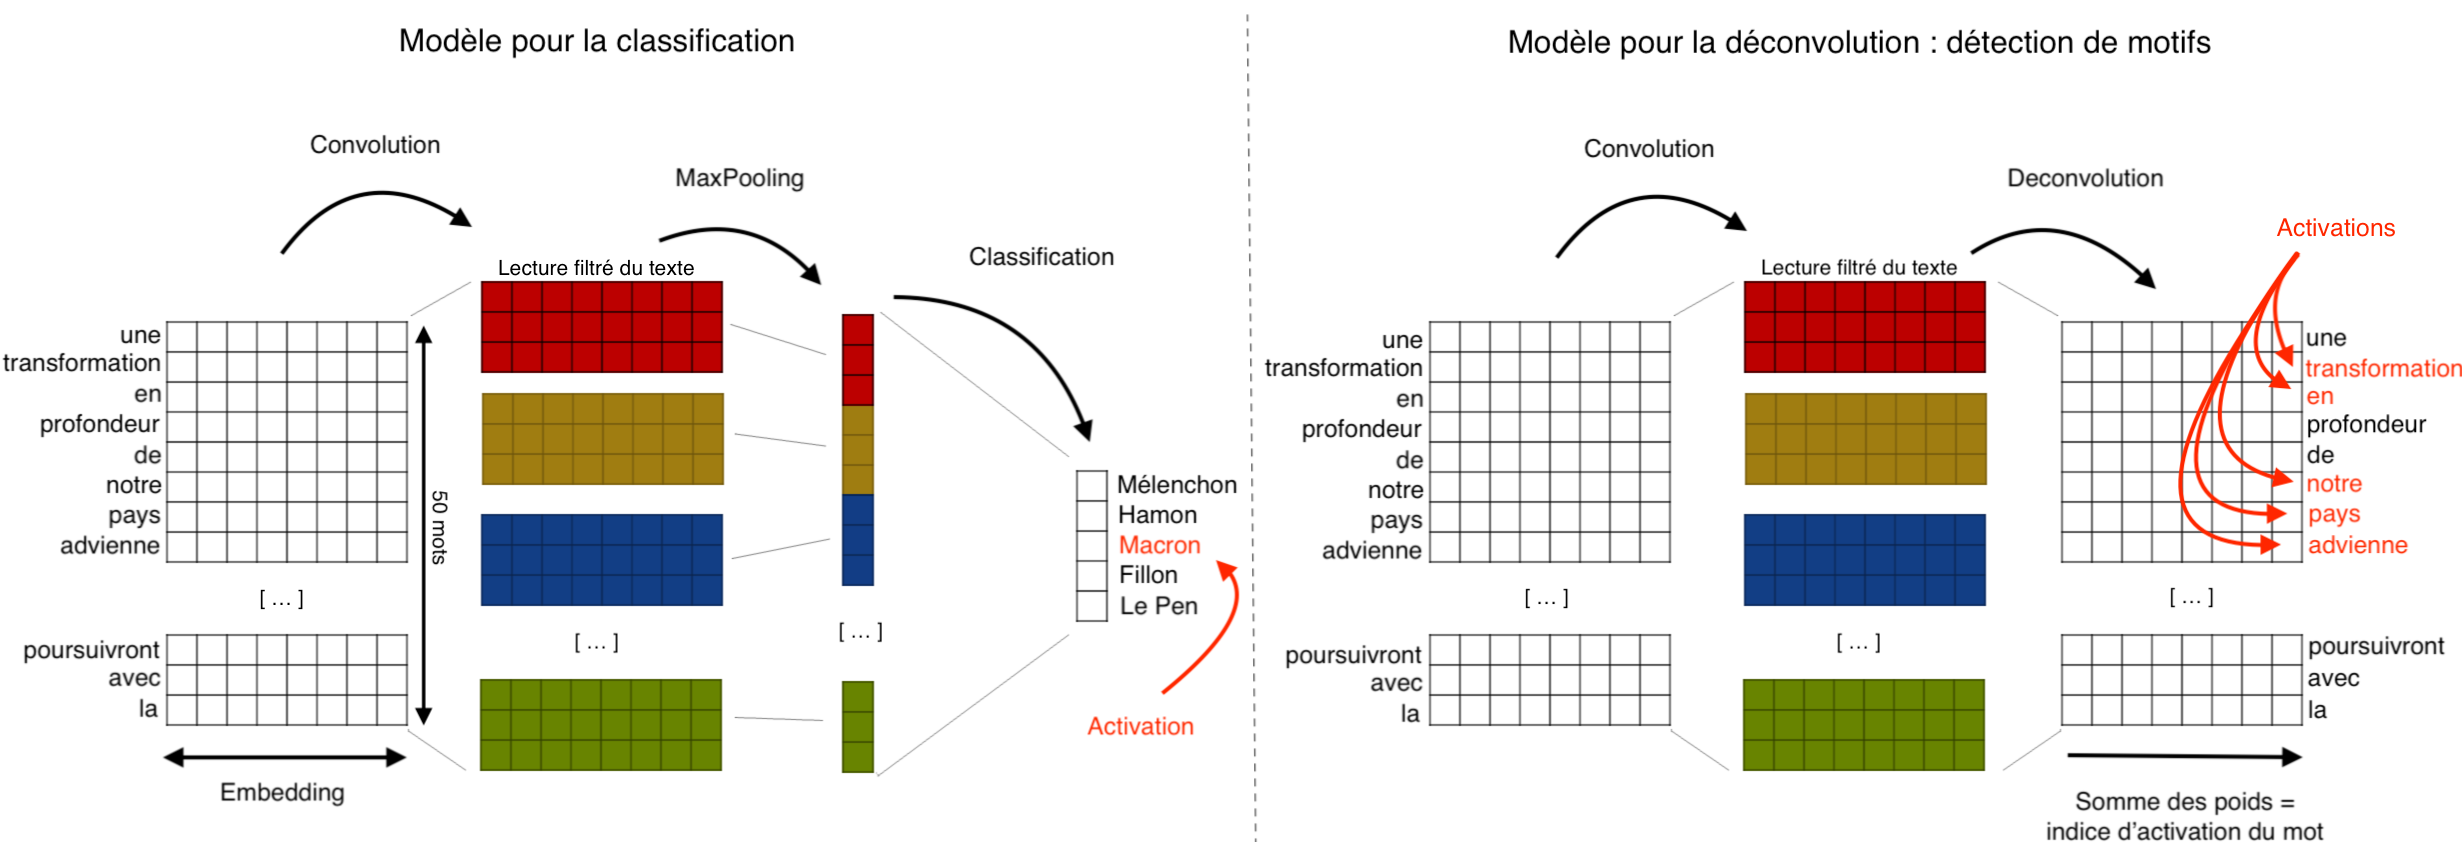
\includegraphics[width=16cm]{img/model.png}
\caption{Deconvolution model}
\label{cnn}
\end{center}
\end{figure}


